\documentclass[10pt]{beamer}

\usetheme{metropolis}
\usepackage{appendixnumberbeamer}

\usepackage{booktabs}
\usepackage[scale=2]{ccicons}
\usepackage{graphicx}
\usepackage{hyperref}
\usepackage{circuitikz}
\usepackage{pdflscape}
\usepackage{smartdiagram}

\usepackage{color}
\usepackage{listings}

\lstset{
	basicstyle=\footnotesize\ttfamily,
    keepspaces=true,
    showstringspaces=false,
    language=PHP,
    commentstyle=\ttfamily,
}

\usepackage[OT4]{polski}
\usepackage[utf8]{inputenc}

\usepackage{pgfplots}
\usepgfplotslibrary{dateplot}

\usepackage{xspace}
\newcommand{\themename}{\textbf{\textsc{metropolis}}\xspace}

\setbeamertemplate{frame footer}{}
\setbeamertemplate{frame numbering}{}

\usetikzlibrary{shapes,arrows}

\tikzstyle{decision} = [diamond, draw, fill=blue!20, 
    text width=4.5em, text badly centered, node distance=3cm, inner sep=0pt]
\tikzstyle{block} = [rectangle, draw, fill=blue!20, 
    text width=5em, text centered, rounded corners, minimum height=4em]
\tikzstyle{line} = [draw, -latex']
\tikzstyle{cloud} = [draw, ellipse,fill=red!20, node distance=3cm,
    minimum height=2em]


\title{Rozszerzanie systemów internetowych}

\subtitle{Projektowanie i programowanie systemów internetowych I}
\author{mgr inż. Krzysztof Rewak}
\date{\today}
\institute{Wydział Nauk Technicznych i Ekonomicznych \\ Państwowa Wyższa Szkoła Zawodowa im. Witelona w Legnicy}

\begin{document}

\maketitle

\begin{frame}{Plan prezentacji}
  \setbeamertemplate{section in toc}[sections numbered]
  \tableofcontents[hideallsubsections]
\end{frame}


\section{Skalowanie systemów}

\begin{frame}{System}	
	Czym jest \textbf{system}?
	
	W teorii systemów jest to zespół elementów realizujący pewną określoną funkcję.
\end{frame}

\begin{frame}{System}	
	Czym jest \textbf{system}?
	
	W rozumieniu systemów internetowych jest to zestaw serwisów tworzących aplikację.
\end{frame}

\begin{frame}[fragile]{Budowa klasycznego systemu internetowego}
	\begin{tikzpicture}[node distance=3cm, minimum size=2cm, auto]
	
		\node [block] (core) {jądro systemu};
	
		\node [block, above of=core] (server) {funkcje serwerowe};
		\node [block, left of=core] (database) {bazy danych};
		\node [block,above left of=core] (cache) {serwery cache};
		\node [block, below left of=core] (filesystem) {systemy plików};
		\node [block, below of=core] (services) {inne serwisy};
	
		\path [line] (core) -- node {} (server);
		\path [line] (server) -- node {} (core);
	
		\path [line] (core) -- node {} (database);
		\path [line] (database) -- node {} (core);
	
		\path [line] (core) -- node {} (cache);
		\path [line] (cache) -- node {} (core);
	
		\path [line] (core) -- node {} (filesystem);
		\path [line] (filesystem) -- node {} (core);
	
		\path [line] (core) -- node {} (services);
		\path [line] (services) -- node {} (core);
		
		\node [circle, fill=orange,inner sep=3pt, right of=core] (http) {serwer HTTP};
	
		\path [line] (http) -- node {} (core);
		\path [line] (core) -- node {} (http);
		
		\node [block, above right of=http] (browser) {przeglądarka};
		\node [block, below right of=http] (api) {inna aplikacja};
	
		\path [line] (http) -- node {} (browser);
		\path [line] (browser) -- node {} (http);
	
		\path [line] (http) -- node {} (api);
		\path [line] (api) -- node {} (http);
	\end{tikzpicture}
\end{frame}

\begin{frame}{Skalowanie}	
	Czym jest \textbf{skalowanie}?
	
	W matematyce możemy powiedzieć o działaniu mnożenia wektora $V$ przez skalar $K$ (jako funkcję $K \times V \rightarrow V$).
\end{frame}

\begin{frame}{Skalowanie}	
	Czym jest \textbf{skalowanie}?
	
	W systemach internetowych chodzi o możliwość zwiększenia skali działania systemu.
\end{frame}

\begin{frame}{Jak skalować?}	
	Skalowanie systemów IT można podzielić na dwa podstawowe typy:
	\begin{itemize}
	\item poziome, \emph{scale-out}, w bok;
	\item pionowe, \emph{scale-up}, w górę.
	\end{itemize}
\end{frame}

\begin{frame}{Skalowanie w górę}	
	Skalowanie w górę jest rozwiązaniem doraźnym, relatywnie łatwym do zastosowania, ale w na dłuższą metę kosztowniejszym.
\end{frame}

\begin{frame}{Skalowanie w górę}	
	Skalowanie w górę polega na zwiększaniu zasobów pod względem ich parametrów. 
	
	Przykładowo jest to dokupienie i instalacja:
	\begin{itemize}
	\item mocniejszego procesora,
	\item mocniejszej karty graficznej,
	\item większego dysku twardego.
	\end{itemize}
\end{frame}

\begin{frame}{Skalowanie w górę}	
	Skalowanie w górę może być łatwym rozwiązaniem problemów.
	
	Przykładowo jest to dokupienie i instalacja:
	\begin{itemize}
	\item kończy się miejsce na dysku? zwiększmy limity!
	\item procesor nie wyrabia? podkręćmy go!
	\end{itemize}
\end{frame}

\begin{frame}[fragile]{Budowa klasycznego systemu internetowego}
	\begin{tikzpicture}[node distance=3cm, minimum size=2cm, auto]
	
		\node [block] (core) {jądro systemu};
	
		\node [block, above of=core] (server) {funkcje serwerowe};
		\node [block, left of=core] (database) {bazy danych};
		\node [block,above left of=core, fill=red] (cache) {serwery cache};
		\node [block, below left of=core, fill=red] (filesystem) {systemy plików};
		\node [block, below of=core] (services) {inne serwisy};
	
		\path [line] (core) -- node {} (server);
		\path [line] (server) -- node {} (core);
	
		\path [line] (core) -- node {} (database);
		\path [line] (database) -- node {} (core);
	
		\path [line] (core) -- node {} (cache);
		\path [line] (cache) -- node {} (core);
	
		\path [line] (core) -- node {} (filesystem);
		\path [line] (filesystem) -- node {} (core);
	
		\path [line] (core) -- node {} (services);
		\path [line] (services) -- node {} (core);
		
		\node [circle, fill=orange,inner sep=3pt, right of=core] (http) {serwer HTTP};
	
		\path [line] (http) -- node {} (core);
		\path [line] (core) -- node {} (http);
		
		\node [block, above right of=http] (browser) {przeglądarka};
		\node [block, below right of=http] (api) {inna aplikacja};
	
		\path [line] (http) -- node {} (browser);
		\path [line] (browser) -- node {} (http);
	
		\path [line] (http) -- node {} (api);
		\path [line] (api) -- node {} (http);
	\end{tikzpicture}
\end{frame}

\begin{frame}[fragile]{Budowa klasycznego systemu internetowego}
	\begin{tikzpicture}[node distance=3cm, minimum size=2cm, auto]
	
		\node [block] (core) {jądro systemu};
	
		\node [block, above of=core] (server) {funkcje serwerowe};
		\node [block, left of=core] (database) {bazy danych};
		\node [block,above left of=core] (cache) {większe serwery cache};
		\node [block, below left of=core] (filesystem) {większe systemy plików};
		\node [block, below of=core] (services) {inne serwisy};
	
		\path [line] (core) -- node {} (server);
		\path [line] (server) -- node {} (core);
	
		\path [line] (core) -- node {} (database);
		\path [line] (database) -- node {} (core);
	
		\path [line] (core) -- node {} (cache);
		\path [line] (cache) -- node {} (core);
	
		\path [line] (core) -- node {} (filesystem);
		\path [line] (filesystem) -- node {} (core);
	
		\path [line] (core) -- node {} (services);
		\path [line] (services) -- node {} (core);
		
		\node [circle, fill=orange,inner sep=3pt, right of=core] (http) {serwer HTTP};
	
		\path [line] (http) -- node {} (core);
		\path [line] (core) -- node {} (http);
		
		\node [block, above right of=http] (browser) {przeglądarka};
		\node [block, below right of=http] (api) {inna aplikacja};
	
		\path [line] (http) -- node {} (browser);
		\path [line] (browser) -- node {} (http);
	
		\path [line] (http) -- node {} (api);
		\path [line] (api) -- node {} (http);
	\end{tikzpicture}
\end{frame}

\begin{frame}{Skalowanie w górę}
	Niestety początkowe niskie koszty stosowania skalowania w górę przeradzają się z czasem w problemy z wydajnością, wzrost stałych kosztów oraz barierę technologiczną.
\end{frame}

\begin{frame}{Skalowanie w bok}
	Skalowanie w bok jest rozwiązaniem długoterminowym, niekiedy nieco trudniejszym w implementacji, ale ostatecznie zazwyczaj zalecanym.
\end{frame}

\begin{frame}{Skalowanie w bok}
	Skalowanie w bok polega na zwiększaniu zasobów pod względem ich liczby. 
	
	Przykładowo jest to dokupienie i instalacja:
	\begin{itemize}
	\item nowego procesora,
	\item nowej karty graficznej,
	\item nowego dysku twardego.
	\end{itemize}
\end{frame}

\begin{frame}[fragile]{Budowa klasycznego systemu internetowego}
	\begin{tikzpicture}[node distance=3cm, minimum size=2cm, auto]
	
		\node [block] (core) {jądro systemu};
	
		\node [block, above of=core] (server) {funkcje serwerowe};
		\node [block, left of=core] (database) {bazy danych};
		\node [block,above left of=core, fill=red] (cache) {serwery cache};
		\node [block, below left of=core, fill=red] (filesystem) {systemy plików};
		\node [block, below of=core] (services) {inne serwisy};
	
		\path [line] (core) -- node {} (server);
		\path [line] (server) -- node {} (core);
	
		\path [line] (core) -- node {} (database);
		\path [line] (database) -- node {} (core);
	
		\path [line] (core) -- node {} (cache);
		\path [line] (cache) -- node {} (core);
	
		\path [line] (core) -- node {} (filesystem);
		\path [line] (filesystem) -- node {} (core);
	
		\path [line] (core) -- node {} (services);
		\path [line] (services) -- node {} (core);
		
		\node [circle, fill=orange,inner sep=3pt, right of=core] (http) {serwer HTTP};
	
		\path [line] (http) -- node {} (core);
		\path [line] (core) -- node {} (http);
		
		\node [block, above right of=http] (browser) {przeglądarka};
		\node [block, below right of=http] (api) {inna aplikacja};
	
		\path [line] (http) -- node {} (browser);
		\path [line] (browser) -- node {} (http);
	
		\path [line] (http) -- node {} (api);
		\path [line] (api) -- node {} (http);
	\end{tikzpicture}
\end{frame}

\begin{frame}[fragile]{Budowa klasycznego systemu internetowego}
	\begin{tikzpicture}[node distance=3cm, minimum size=2cm, auto]
	
		\node [block] (core) {jądro systemu};
	
		\node [block, above of=core] (server) {funkcje serwerowe};
		\node [block, left of=core] (database) {bazy danych};
		\node [block, above left of=core] (cache) {serwery cache};
		\node [block, below left of=core] (filesystem) {systemy plików};
		\node [block, below of=core] (services) {inne serwisy};
		\node [block, above right of=core] (cache) {nowe serwery cache};
		\node [block, below right of=core] (filesystem) {nowe systemy plików};
	
		\path [line] (core) -- node {} (server);
		\path [line] (server) -- node {} (core);
	
		\path [line] (core) -- node {} (database);
		\path [line] (database) -- node {} (core);
	
		\path [line] (core) -- node {} (cache);
		\path [line] (cache) -- node {} (core);
	
		\path [line] (core) -- node {} (filesystem);
		\path [line] (filesystem) -- node {} (core);
	
		\path [line] (core) -- node {} (services);
		\path [line] (services) -- node {} (core);
		
		\node [circle, fill=orange,inner sep=3pt, right of=core] (http) {serwer HTTP};
	
		\path [line] (http) -- node {} (core);
		\path [line] (core) -- node {} (http);
		
		\node [block, above right of=http] (browser) {przeglądarka};
		\node [block, below right of=http] (api) {inna aplikacja};
	
		\path [line] (http) -- node {} (browser);
		\path [line] (browser) -- node {} (http);
	
		\path [line] (http) -- node {} (api);
		\path [line] (api) -- node {} (http);
	\end{tikzpicture}
\end{frame}

\begin{frame}{Skalowanie w bok}
	Skalowanie w bok jest łatwe i z czasem mniej kosztowne od skalowania w górę, jednakże jest trudniejsze w implementacji.
\end{frame}

\begin{frame}{Skok w bok}
	Przykładowo jak rozpraszać dane na kilka baz danych?
\end{frame}

\section{Automatyzacja wdrażania systemów}

\begin{frame}{Jak wdrożyć system internetowy?}
	Przy wdrażaniu projektu można obrać wiele dróg. Między innymi:
	
	\begin{itemize}
	\item zbudować go w pełni na maszynie deweloperskiej i przesłać przez FTP? (brzmi okropnie)
	\item wykorzystać system kontroli wersji, skorzystać z SSH i odpalić wszystko, co trzeba na maszynie produkcyjnej (nieco lepiej, ale też może boleć)
	\item oskryptować wszystko i uruchomić wdrożenie pod jednym przyciskiem.
	\end{itemize}
\end{frame}

\begin{frame}{Jak wdrożyć system internetowy?}
	\emph{Continuous integration}, \textbf{CI}, czyli \emph{ciągła integracja} to jedna z części \emph{extreme programming}, zaraz obok testów jednostkowych, programowania parami czy stand-upów.
\end{frame}

\begin{frame}{Dobre praktyki CI}
	Na \emph{continuous integration} składa się kilka dobrych praktyk, o których warto wspomnieć.
\end{frame}

\begin{frame}{Dobre praktyki CI}
	Korzystanie z systemu kontroli wersji to podstawa. VCS powinien zarządzać repozytoriami z kodem aplikacji. Główna gałąź repozytorium powinna zawierać najaktualniejszą wersję aplikacji.
	
	Jeżeli to potrzebne, należy zautomatyzować proces budowania aplikacji. Tutaj warto zapoznać się z oprogramowaniem takim jak Travis, Jenkis lub Gitlab.
\end{frame}

\begin{frame}{Dobre praktyki CI}
	Kod powinien być otestowany, a środowisko testów uruchamiane automatycznie. Przed wdrożeniem nie może się okazać, że niektóre części aplikacji działają w sposób inny niż oczekiwany.
	
	W teorii każda zmiana powinna trafiać na główną gałąź repozytorium codziennie. Każdy commit powinien również inicjować proces budowania aplikacji.
\end{frame}

\begin{frame}{Dobre praktyki CI}
	Proces integracji powinien być szybki.
	
	Testy powinny odbywać się w specjlanym środowisku. Może się ono nieznacznie różnić od produkcyjnego (przede wszystkim skalą), lecz idealnie byłoby wykorzystanie konteneryzacji lub wirtualizacji do maksymalnego zbliżenia warunków środowiskowych.
\end{frame}

\begin{frame}{Dobre praktyki CI}
	Każdy powinien móc zobaczyć status ostatnich akcji. Mowa zarówno o testach automatycznych, pobraniu zależności, budowaniu aplikacji i innych funkcjonalnościach.
	
	Wykorzystać \emph{continuous deployment}, czyli pełne zutomatyzowanie procesu wdrażania aplikacji. 
\end{frame}

\begin{frame}{CD}
	\begin{figure}[t]
		\centering
		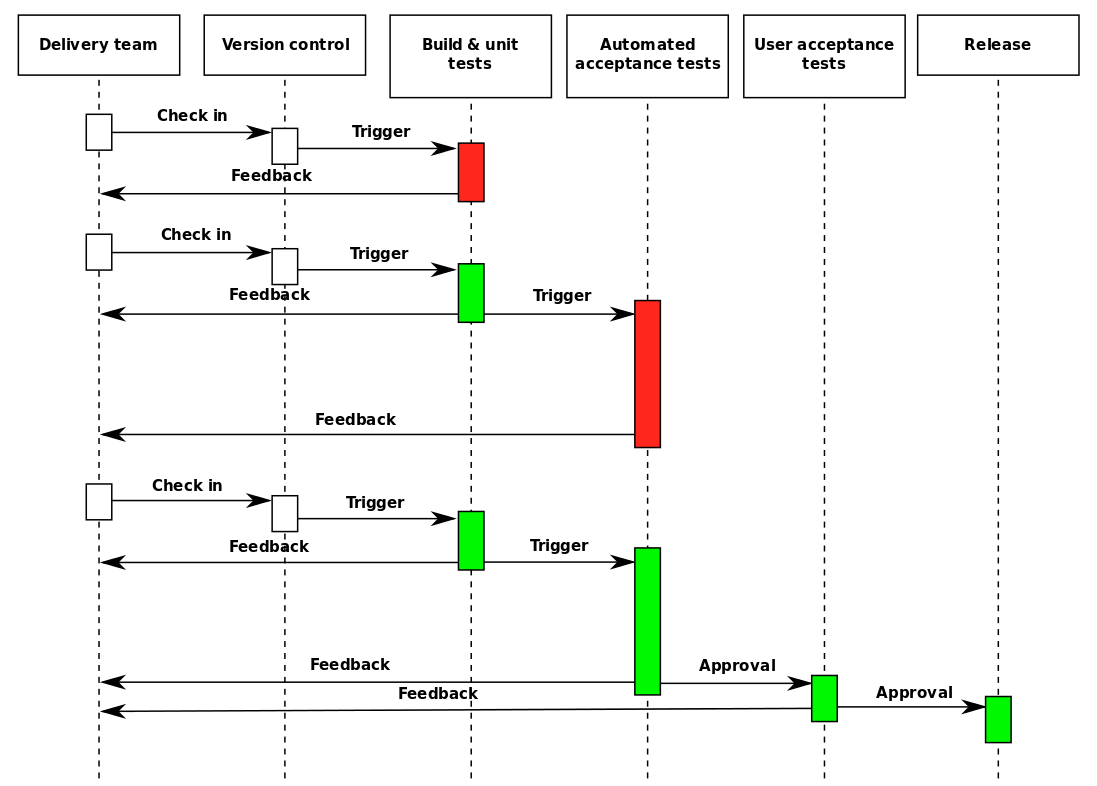
\includegraphics[width=\linewidth]{cd.png}
	\end{figure}
\end{frame}

\section{Podsumowanie}

\begin{frame}{Bibliografia i ciekawe źródła}
  
	\begin{thebibliography}{9}
		
		\bibitem{ci}
		\url{https://en.wikipedia.org/wiki/Continuous_integration}
		
		\bibitem{cd}
		\url{https://en.wikipedia.org/wiki/Continuous_delivery}
		
	\end{thebibliography}

\end{frame}

\appendix

\begin{frame}[standout]
	Pytania?
\end{frame}

\begin{frame}{}

	Kod prezentacji dostępny jest w repozytorium git pod adresem \texttt{https://bitbucket.org/krewak/pwsz-ppsi} \\ \ \\

	\begin{figure}
		\centering
		\href{https://bitbucket.org/krewak/pwsz-ppsi}{
			
\includegraphics[width=.15\textwidth]{../_template/bitbucket.png}
		}
	\end{figure}
	
	Wszystkie informacje dot. kursu dostępne są pod adresem \texttt{http://pwsz.rewak.pl/kursy/4} \\ \ \\

	\begin{figure}
		\centering
		\href{http://pwsz.rewak.pl/kursy/3}{
			
\includegraphics[width=.15\textwidth]{../_template/rewak.png}
		}
	\end{figure}

\end{frame}

\end{document}
